\chapter{HLT description and efficiency}\label{appendix:ApendiceA}

\section{Trigger Paths}

In the analysis we search for a signal with one energetic jet emerging from a boosted boson (Z or W ) and large amount of missing transverse energy ($\MET$). Therefore,  we employ a data sample that was collected using triggers prepared to select events that have $\MET$ and a quantity associated to jets ($H_{\text{T}}^{\text{miss}}$). The main signal trigger path chosen is:
\begin{itemize}
\item
 $\verb|PFMETNoMu90_JetIdCleaned_PFMHTNoMu90_IDTight|$ 
\end{itemize}
The $\MET$(MET) is defined as the negative vectorial sum of the transverse momentum of all the particles in the event and the $H_{\text{T}}^{\text{miss}}$(MHT) is defined as the negative vectorial sum of the transverse momentum of all the jets in the event. Both quantities were calculated using particle flow (PF) objects adding back the vector momenta of all PF muons (NoMu). The main trigger path present thresholds of 90 GeV in $\MET$ and $H_{\text{T}}^{\text{miss}}$. 
In order to prevent collect noise events online that will be discarded offline, some additional requirements are included in the trigger path. They relies on the online application of the jet energy corrections for jets with transverse momentum bigger than 20 GeV, a selection on neutral hadron energy fraction (NHF $<$ 0.9) and tight jet identification conditions in the calculation of the $H_{\text{T}}^{\text{miss}}$.\\ 
In addition an inclusive $\MET$ trigger path is employ (in a OR) with the main signal trigger path:
\begin{itemize}
\item
 $\verb|HLT_PFMET170_*|$
\end{itemize}
This path act as a support trigger to gain acceptance at high $\MET$ to recover inefficiency of the main trigger path. The missing transverse
momentum threshold applied in the online selection is 170 GeV, where the $\MET$ is calculated  using the PF algorithm.
The signal HLT paths are seeded at level 1 (in a OR) by $\verb|L1ETM50|$, $\verb|L1ETM60|$ and $\verb|L1ETM70|$. 

\section{Trigger Efficiency}

In order to measured the trigger efficiency in data we use the reference trigger method with an unbiased data sample of single muon events, collected with the trigger path $\verb|HLT_IsoMu20_v*|$ and  grouped in the Primary Dataset SingleMu. 
For the measurement of the efficiency in MC an inclusive W + jets sample was used.

For the offline selection we impose the next conditions in Data and MC:
\begin{itemize}
\item
We require at least one muon with the following properties:
\begin{itemize}
\item 
$\pt >$  10 GeV, $\left| \eta \right| <$ 2.5
\item 
Tight muon ID
\item
Relative isolation with $\Delta \beta$ correction less than 0.15
\end{itemize}
\item
We require at least one ak4jet with the following properties:
\begin{itemize}
\item 
$\pt >$  100 GeV, $\left| \eta \right| <$ 2.5
\item
Loose jet ID
\item
Cleaning cuts : CHF $>$ 0.1, NHF $<$ 0.8
\item
$\Delta R$ (jet,leptons) $>$ 0.5
\end{itemize}
\item
General requirements:
\begin{itemize}
\item 
At least one good offline primary vertex
\item
Events pass the $\MET$ filters
\item
min $\Delta \phi$ ( AK4Jet,$\MET$) $>$ 0.4
\item
$\dfrac{\left|\text{CALO MET - MET} \right|}{\text{MET}} <$ 0.5 
\end{itemize}
\end{itemize}



The performance of the trigger efficiency is measured in Data and MC, using the definition:
\begin{eqnarray}\label{eq1}
\text{efficiency} = \dfrac{ \text{passed} ( \text{HLT$\_$IsoMu20  \&\& } (\text{OR of Signal Triggers})   \text{\&\& Offline Selection} )}{\text{passed} (  \text{HLT$\_$IsoMu20  \&\& }  \text{ Offline Selection})}
\end{eqnarray}

\begin{figure}[!ht]
\begin{center}
  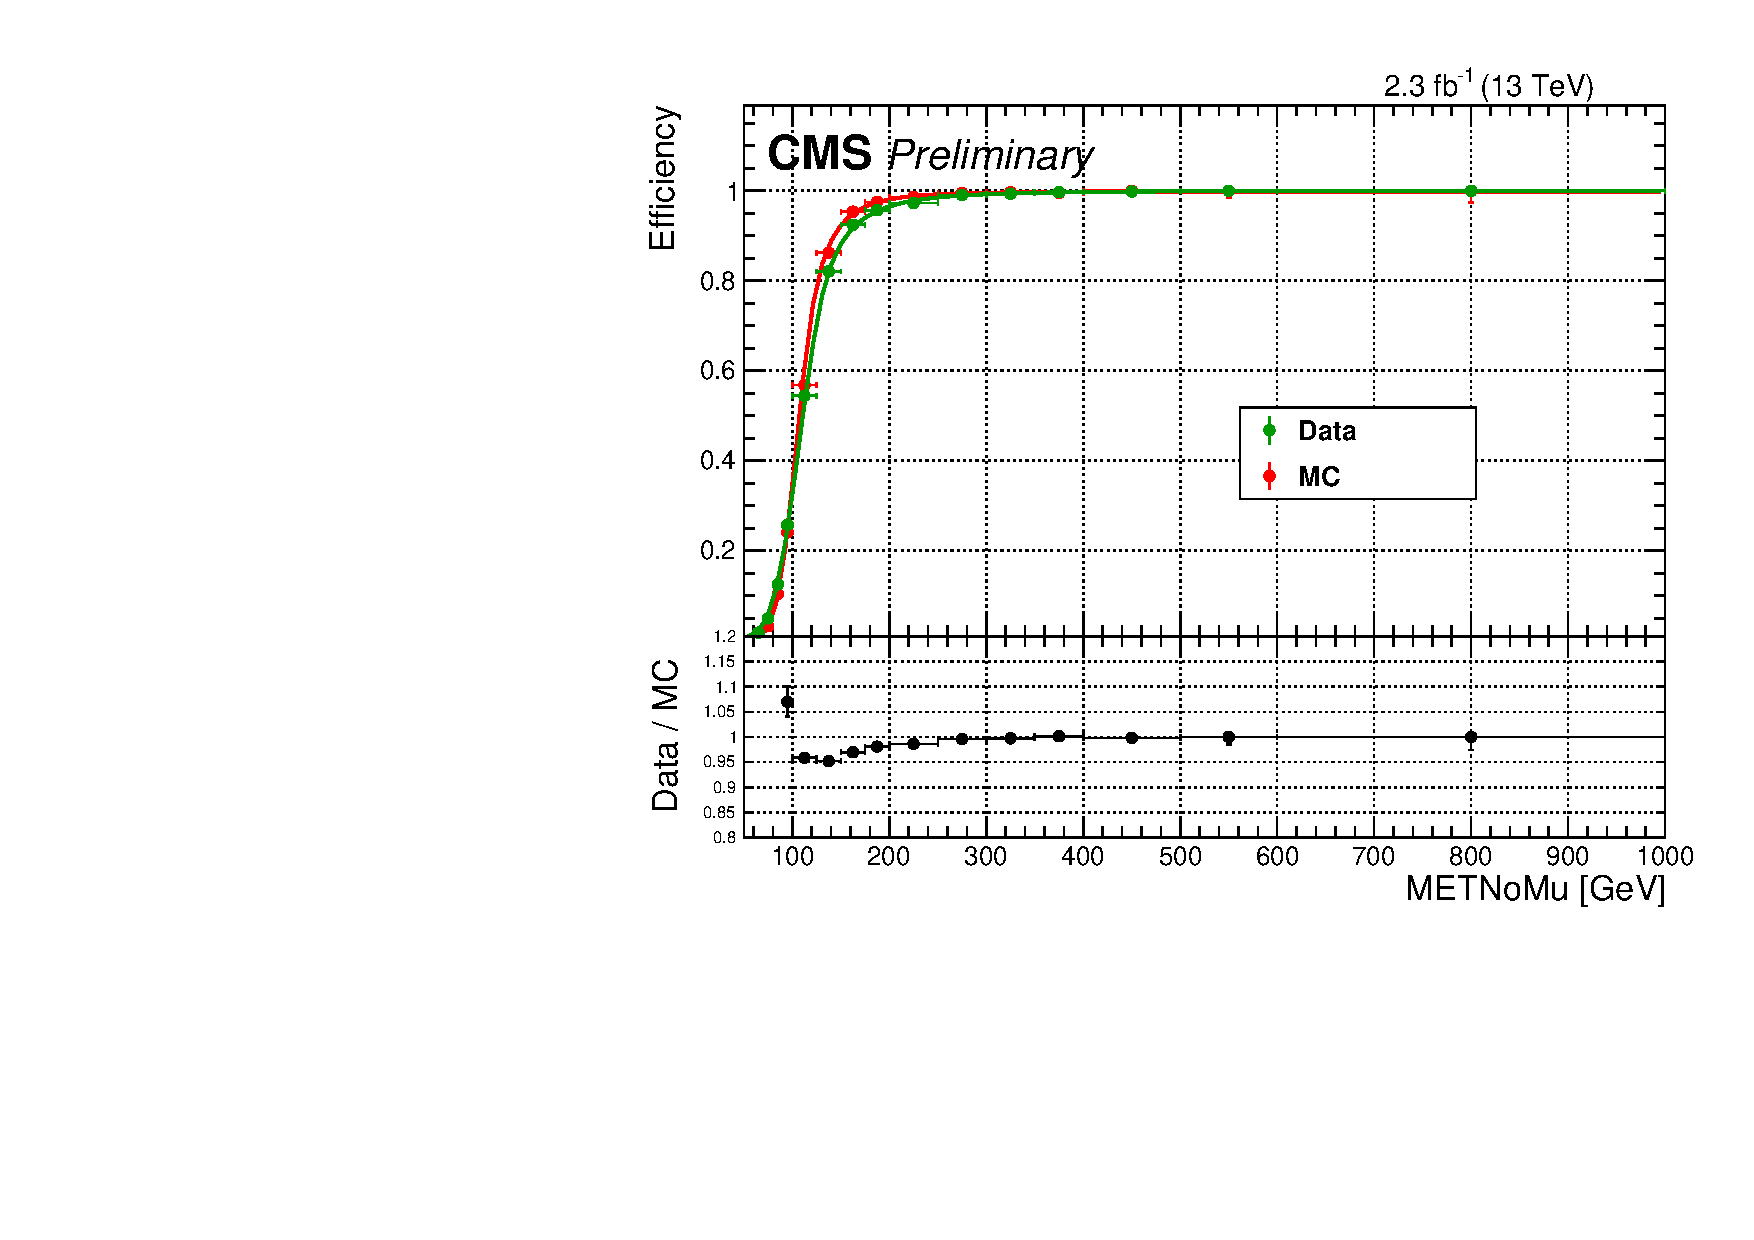
\includegraphics[width=350pt]{figures/trigger/trigeffOct23.pdf}
\end{center}
\caption{High Level Trigger efficiency in function of the transvserse missing energy without muons for the selected paths. The figure shows the turn-on curve for data and MC simulation and the Data/MC ratio.}
\label{fig:TriggerEff1}
\end{figure}

\begin{table}[!ht]
\begin{center}
\caption{Trigger efficiency for different $\MET(\text{NoMu})$ values in Data and MC.}
\label{tab:effvalues}
\begin{tabular}{ccc} \hline
$\MET(\text{NoMu})$ value (GeV) & Trigger efficiency in MC ($\%$)  & Trigger efficiency in Data ($\%$)  \\ \hline
200  &  98 & 96.5 \\
250  &  99.2  & 98.5\\
300  &  99.5 &  99.2 \\
350  &  99.6 &  99.5 \\
400  &  99.7 &  99.7 \\
500  &  99.79 & 99.8   \\
1000  &  99.8 & 100  \\ \hline
\end{tabular}
\end{center}
\end{table}

For events passing the selection $\MET(\text{NoMu}) >$ 250 GeV, the trigger present an efficiency around  99$\%$. 

In the analysis, the trigger decision is applied on both data and MC and residual Data/MC scale factors obtained from the Data/MC ratio are
imposed to the MC with the resulting uncertainty considered later on as systematics.

\section{Crosscheck of trigger efficiency measurement}

As as crosschek of the previous efficiency measurement we will use a SingleElectron data sample for data and a W +jets sample for MC with  the following reference trigger paths:

\begin{itemize}
\item
 $\verb|HLT_Ele32_eta2p1_WPTight_Gsf_v*|$
\item
$\verb|HLT_Ele105_CaloIdVT_GsfTrkIdT_v*|$
\end{itemize}

For the offline selection we impose the next conditions in Data and MC:
\begin{itemize}
\item
We require at least one electron with the following properties:
\begin{itemize}
\item
$\pt >$  40 GeV, $\left| \eta \right| <$ 2.5
\item
Tight electron ID
\end{itemize}
\item
We require at least one ak4jet with the following properties:
\begin{itemize}
\item
$\pt >$  100 GeV, $\left| \eta \right| <$ 2.5
\item
Loose jet ID
\item
Cleaning cuts : CHF $>$ 0.1, NHF $<$ 0.8
\item
$\Delta R$ (jet,leptons) $>$ 0.5
\end{itemize}
\item
General requirements:
\begin{itemize}
\item
At least one good offline primary vertex
\item
Events pass the $\MET$ filters
\item
min $\Delta \phi$ ( AK4Jet,$\MET$) $>$ 0.4
\item
$\dfrac{\left|\text{CALO MET - MET} \right|}{\text{MET}} <$ 0.5
\end{itemize}
\end{itemize}
The performance of the trigger efficiency is measured in Data and MC using a similar definition as the one given in \eqref{eq1}.
In the figure \ref{fig:TriggerEffele} we show the turn-on curve for the high level trigger efficiency in function of the transverse missing energy for data and W+jets events. 

\begin{figure}[!ht]
\begin{center}
  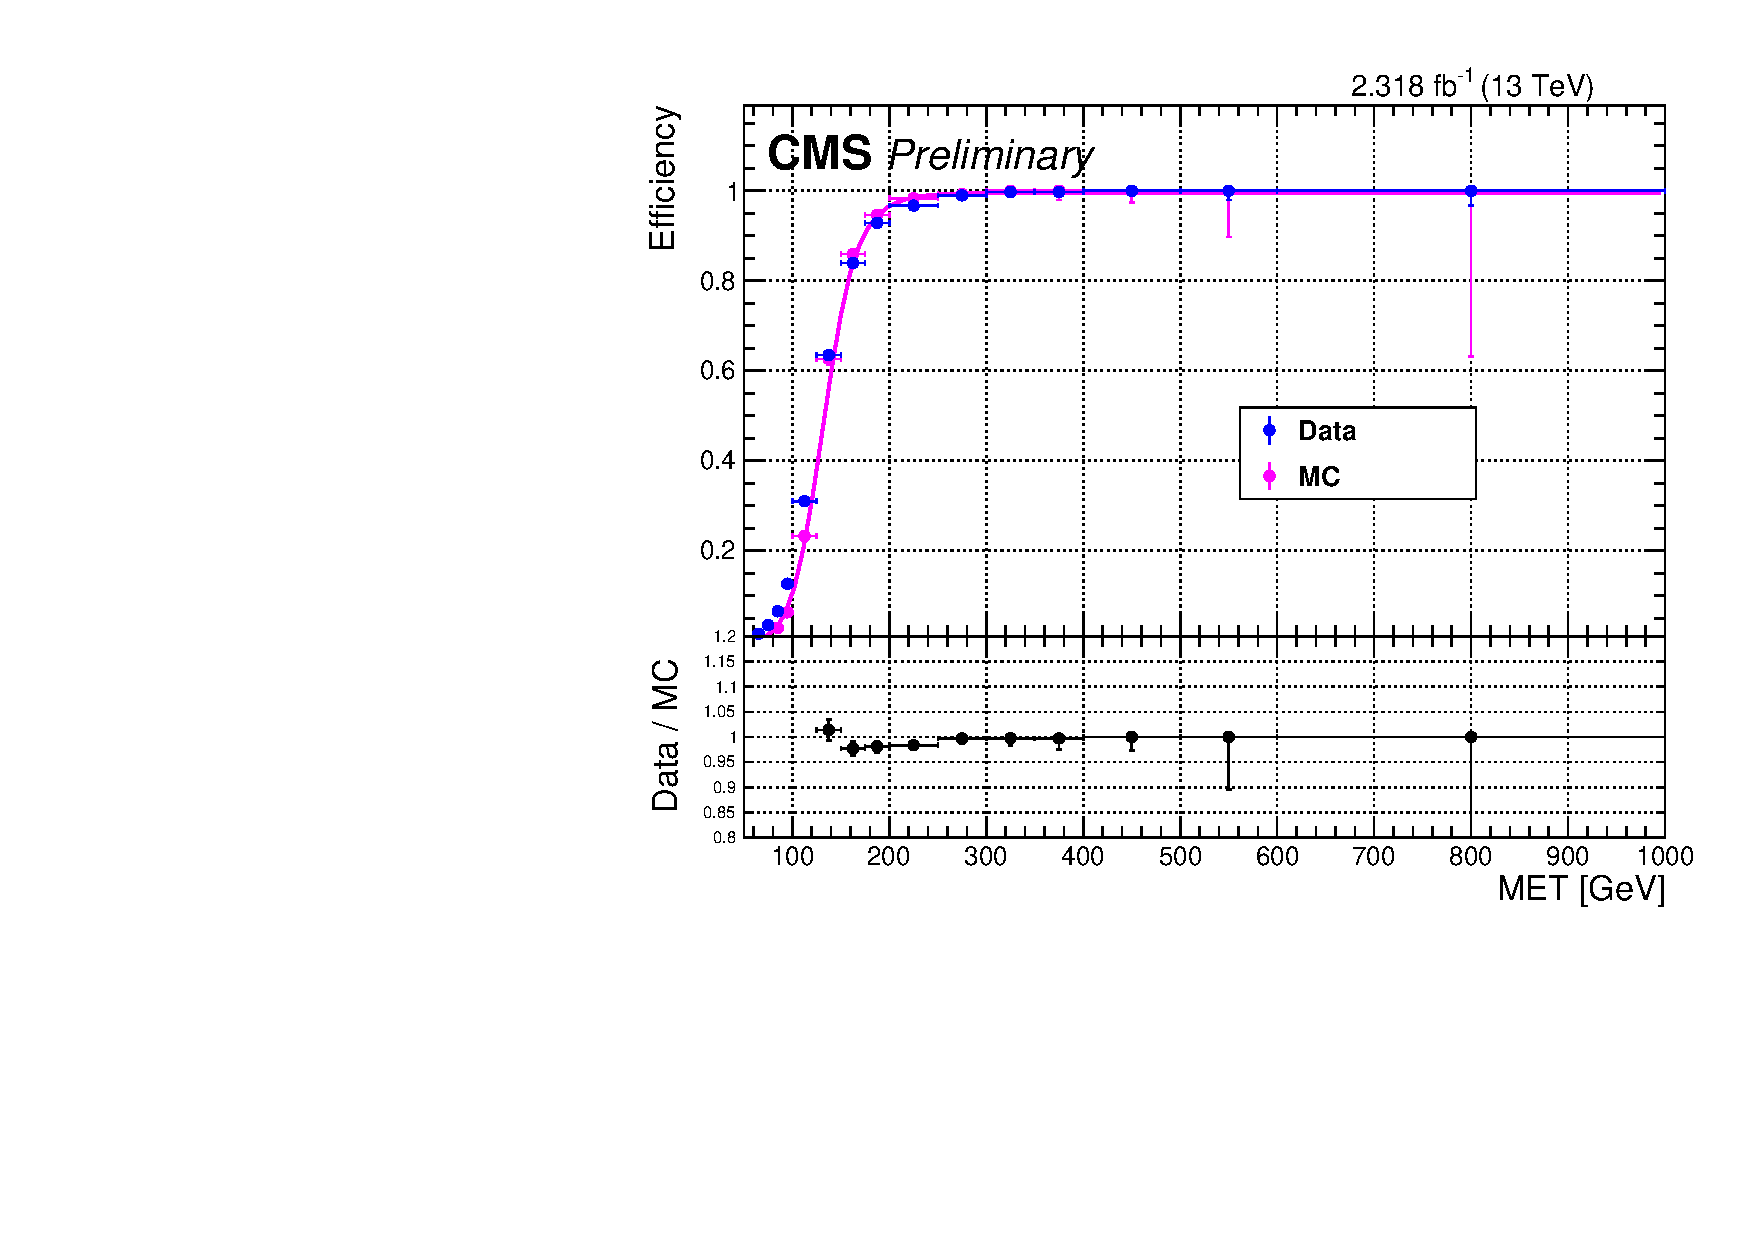
\includegraphics[width=350pt]{figures/trigger/trigeffJul18.pdf}
\end{center}
\caption{High Level Trigger efficiency in function of the transvserse missing energy for the selected paths. The figure shows the turn-on curve for data and MC simulation.}
\label{fig:TriggerEffele}
\end{figure}

\begin{table}[!ht]
\begin{center}
\caption{Trigger efficiency for different $\MET$ values in Data and MC.}
\label{tab:effvalues2}
\begin{tabular}{ccc} \hline
$\MET$ value (GeV) & Trigger efficiency in MC ($\%$)  & Trigger efficiency in Data ($\%$)  \\ \hline
200  &  96.5 & 94.5 \\
250  &  99.1  & 98.5\\
300  &  99.4 &  99.4 \\
350  &  99.46 &  99.7 \\
400  &  99.47 &  99.7 \\
500  &  99.47 & 99.7   \\
1000  &  99.47 & 99.7  \\ \hline
\end{tabular}
\end{center}
\end{table}

For events passing the selection $\MET >$ 250 GeV, the trigger is 99$\%$ efficient.
As can be observed  from the figures \ref{fig:TriggerEff1}, \ref{fig:TriggerEffele} and the tables \ref{tab:effvalues2}, \ref{tab:effvalues}, we obtained similar results for the trigger efficiency using the SingleMu or the SingleElectron dataset. In addition, the figure \ref{fig:TriggerSignal} shows the trigger turn on curves for MC signal samples, where the analysis selection was applied.

\begin{figure}[!ht]
\begin{center}
  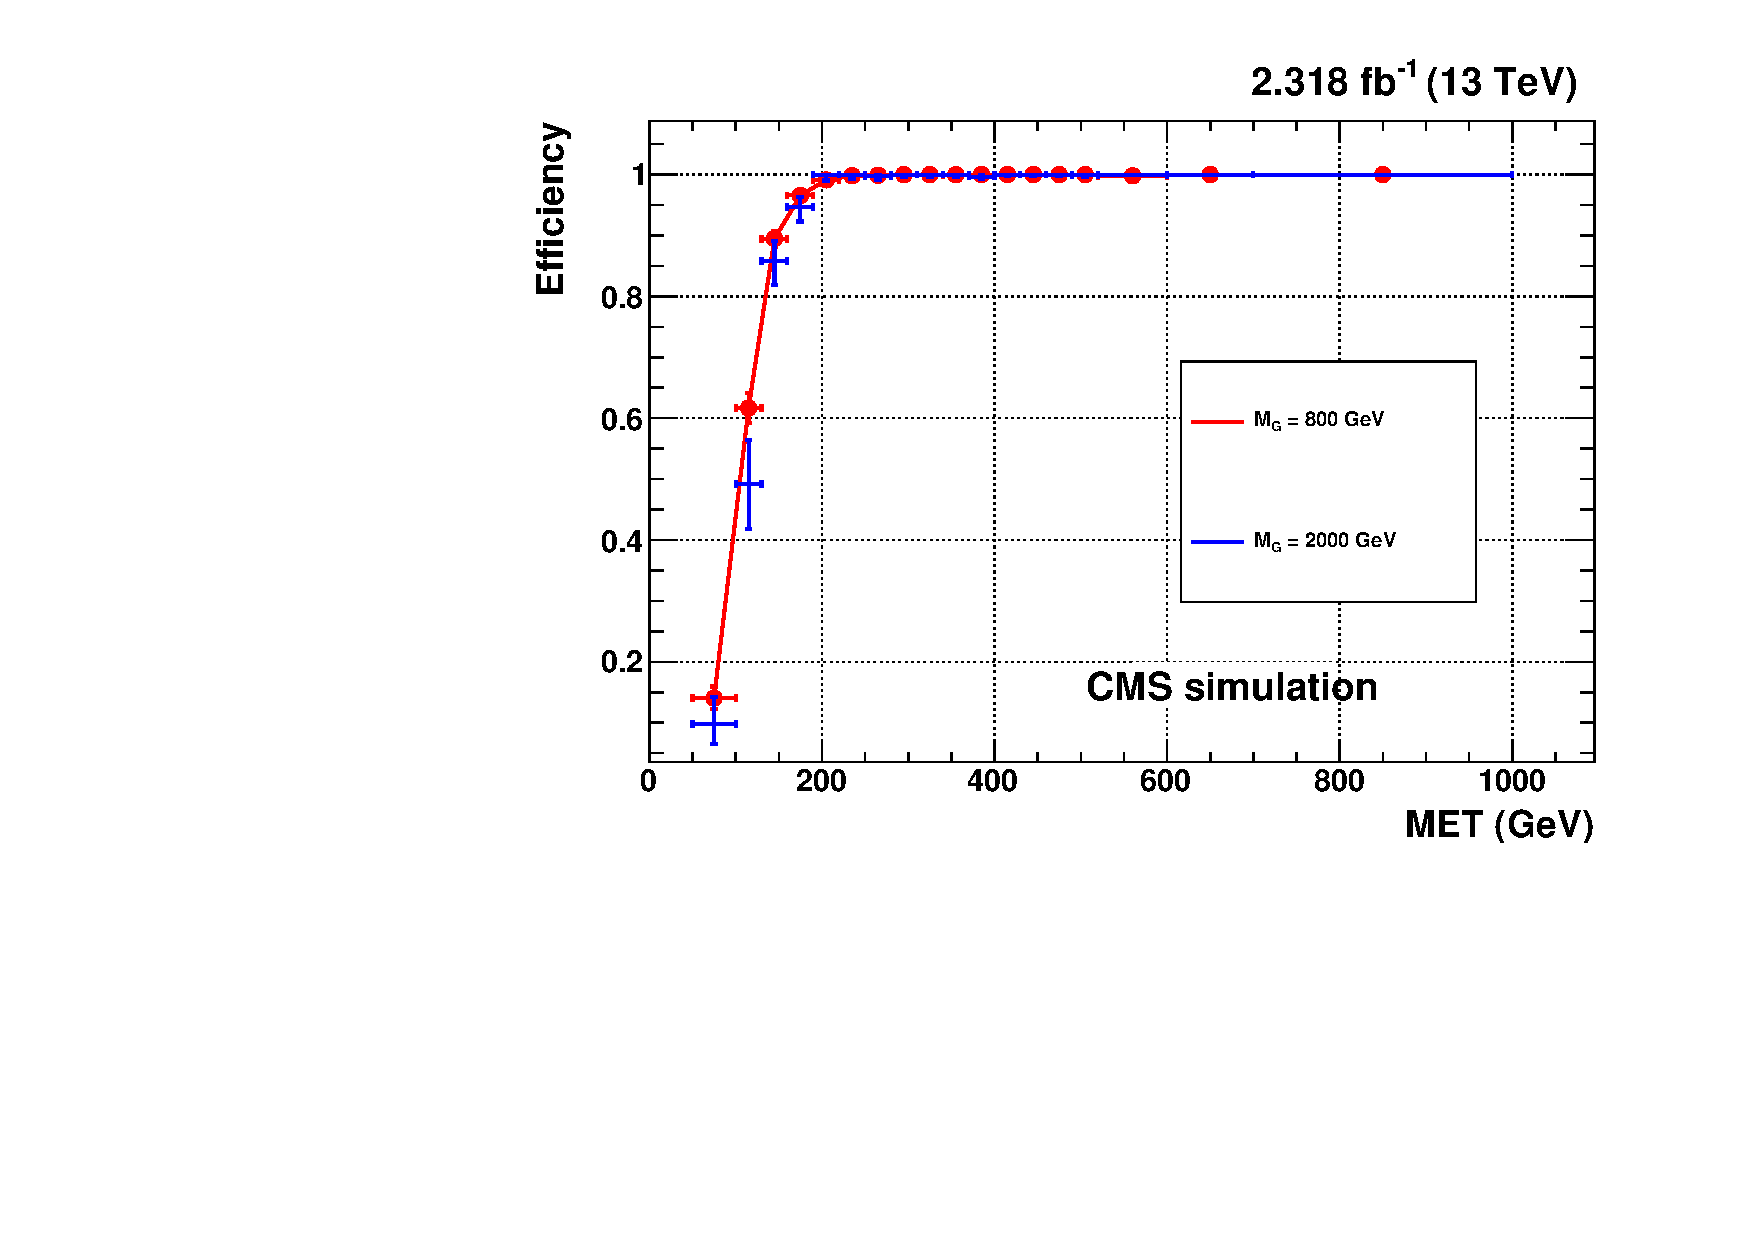
\includegraphics[width=300pt]{figures/trigger/triggerEffcompSignal.pdf}
\end{center}
\caption{High level trigger efficiency in function of the transvserse missing energy for the selected path in RS signal samples. The figure shows the turn-on curve for different mass points.}
\label{fig:TriggerSignal}
\end{figure}





